\documentclass{beamer}

\mode<presentation> {

\usepackage{graphicx}
\usepackage[utf8]{inputenc}
\usepackage[ngerman]{babel}

\usetheme{Boadilla}
\usecolortheme{seagull}

\setbeamertemplate{footline}[page number] % Einfacher Folienzähler als Fußzeile
\setbeamertemplate{navigation symbols}{} % Keine Navigationslinks
}

\defbeamertemplate*{title page}{customized}[1][]
{
  \centering
  \usebeamerfont{title}{\LARGE \inserttitle}\par
  \usebeamerfont{subtitle}\usebeamercolor[fg]{subtitle}\insertsubtitle\par
  \bigskip
  \usebeamercolor[fg]{titlegraphic}\inserttitlegraphic\par
  \bigskip
  \usebeamerfont{author}\insertauthor\\[0.5em]
  \usebeamerfont{institute}\insertinstitute\par
  \usebeamerfont{date}\insertdate\par
}

\title[Lens]{Lenses und Zauberwürfel}
\titlegraphic{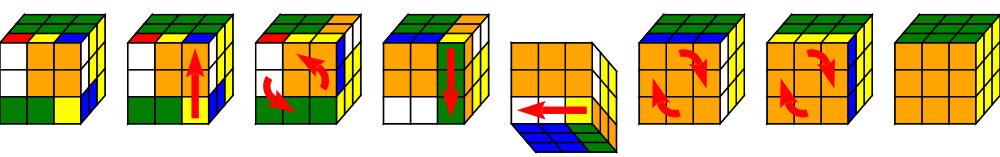
\includegraphics[width=0.65\linewidth]{rubiks-sequence.png}}
\author{Tim Baumann}
\institute[CCA]{Curry Club Augsburg}
\date{13. August 2015}

\begin{document}

\begin{frame}
  \titlepage
\end{frame}

\iffalse
\begin{frame}
  \frametitle{Übersicht}
  \tableofcontents
\end{frame}
\fi

\section{First Section}

\subsection{Subsection Example} % A subsection can be created just before a set of slides with a common theme to further break down your presentation into chunks

\begin{frame}
  \frametitle{Multiple Columns}
  \begin{columns}[c] % The "c" option specifies centered vertical alignment while the "t" option is used for top vertical alignment
    \column{.45\textwidth} % Left column and width
    \textbf{Heading}
    \begin{enumerate}
      \item Statement
      \item Explanation
      \item Example
    \end{enumerate}

    \column{.5\textwidth} % Right column and width
    Lorem ipsum dolor sit amet, consectetur adipiscing elit. Integer lectus nisl, ultricies in feugiat rutrum, porttitor sit amet augue. Aliquam ut tortor mauris. Sed volutpat ante purus, quis accumsan dolor.
  \end{columns}
\end{frame}

\section{Second Section}

\begin{frame}
  \frametitle{Welche Bibliothek?}
  % Bildquelle: https://ro-che.info/ccc/23
  \begin{figure}
    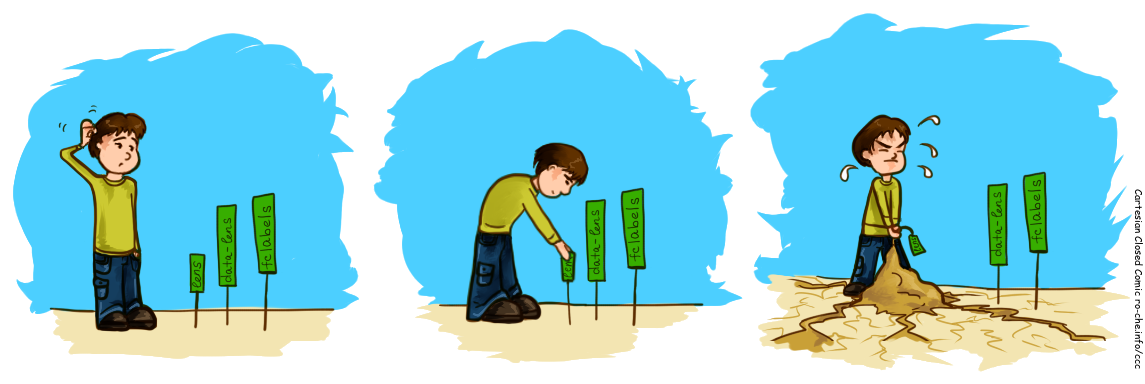
\includegraphics[width=0.9\linewidth]{ccc-picking-lens-library.png}
    \caption{Picking a Lens Library (Cartesian Closed Comic)}
  \end{figure}
\end{frame}

\end{document}
